
\section{Prototyp zapojenia pomocou jednostrannej prototypovej dosky}

Ako ovládací prvok v 2. generácii obr.\ref{OBRAZOK 1.5} systému sme si zvolili Arduino pro mini, ktorého rozmery a cena boli vyhovujúce pre naše potreby. Schéma zapojenia pre Arduino pro mini je totožná so zapojením pre Arduino UNO až na to, že Arduino pro mini sme sa rozhodli napájať pomocou 3,7V lítiovej batérie zapojenej v kontrolóri nabíjania batérie 03962A. Na správne fungovanie lítiovej batérie je kritické nedovoliť batérii úplne sa vybiť. Z tohto dôvodu budeme pomocou analógového pinu A2, merať napätie batérie a pri kritickom napätí sa spustí blikanie led diódy obr.\ref{OBRAZOK 1.7}, ktorá indikuje nutnosť nabitia batérie pomocou mikro USB portu obr.\ref{OBRAZOK 1.6}.

\begin{figure}[!tbh]
\centering
\fbox{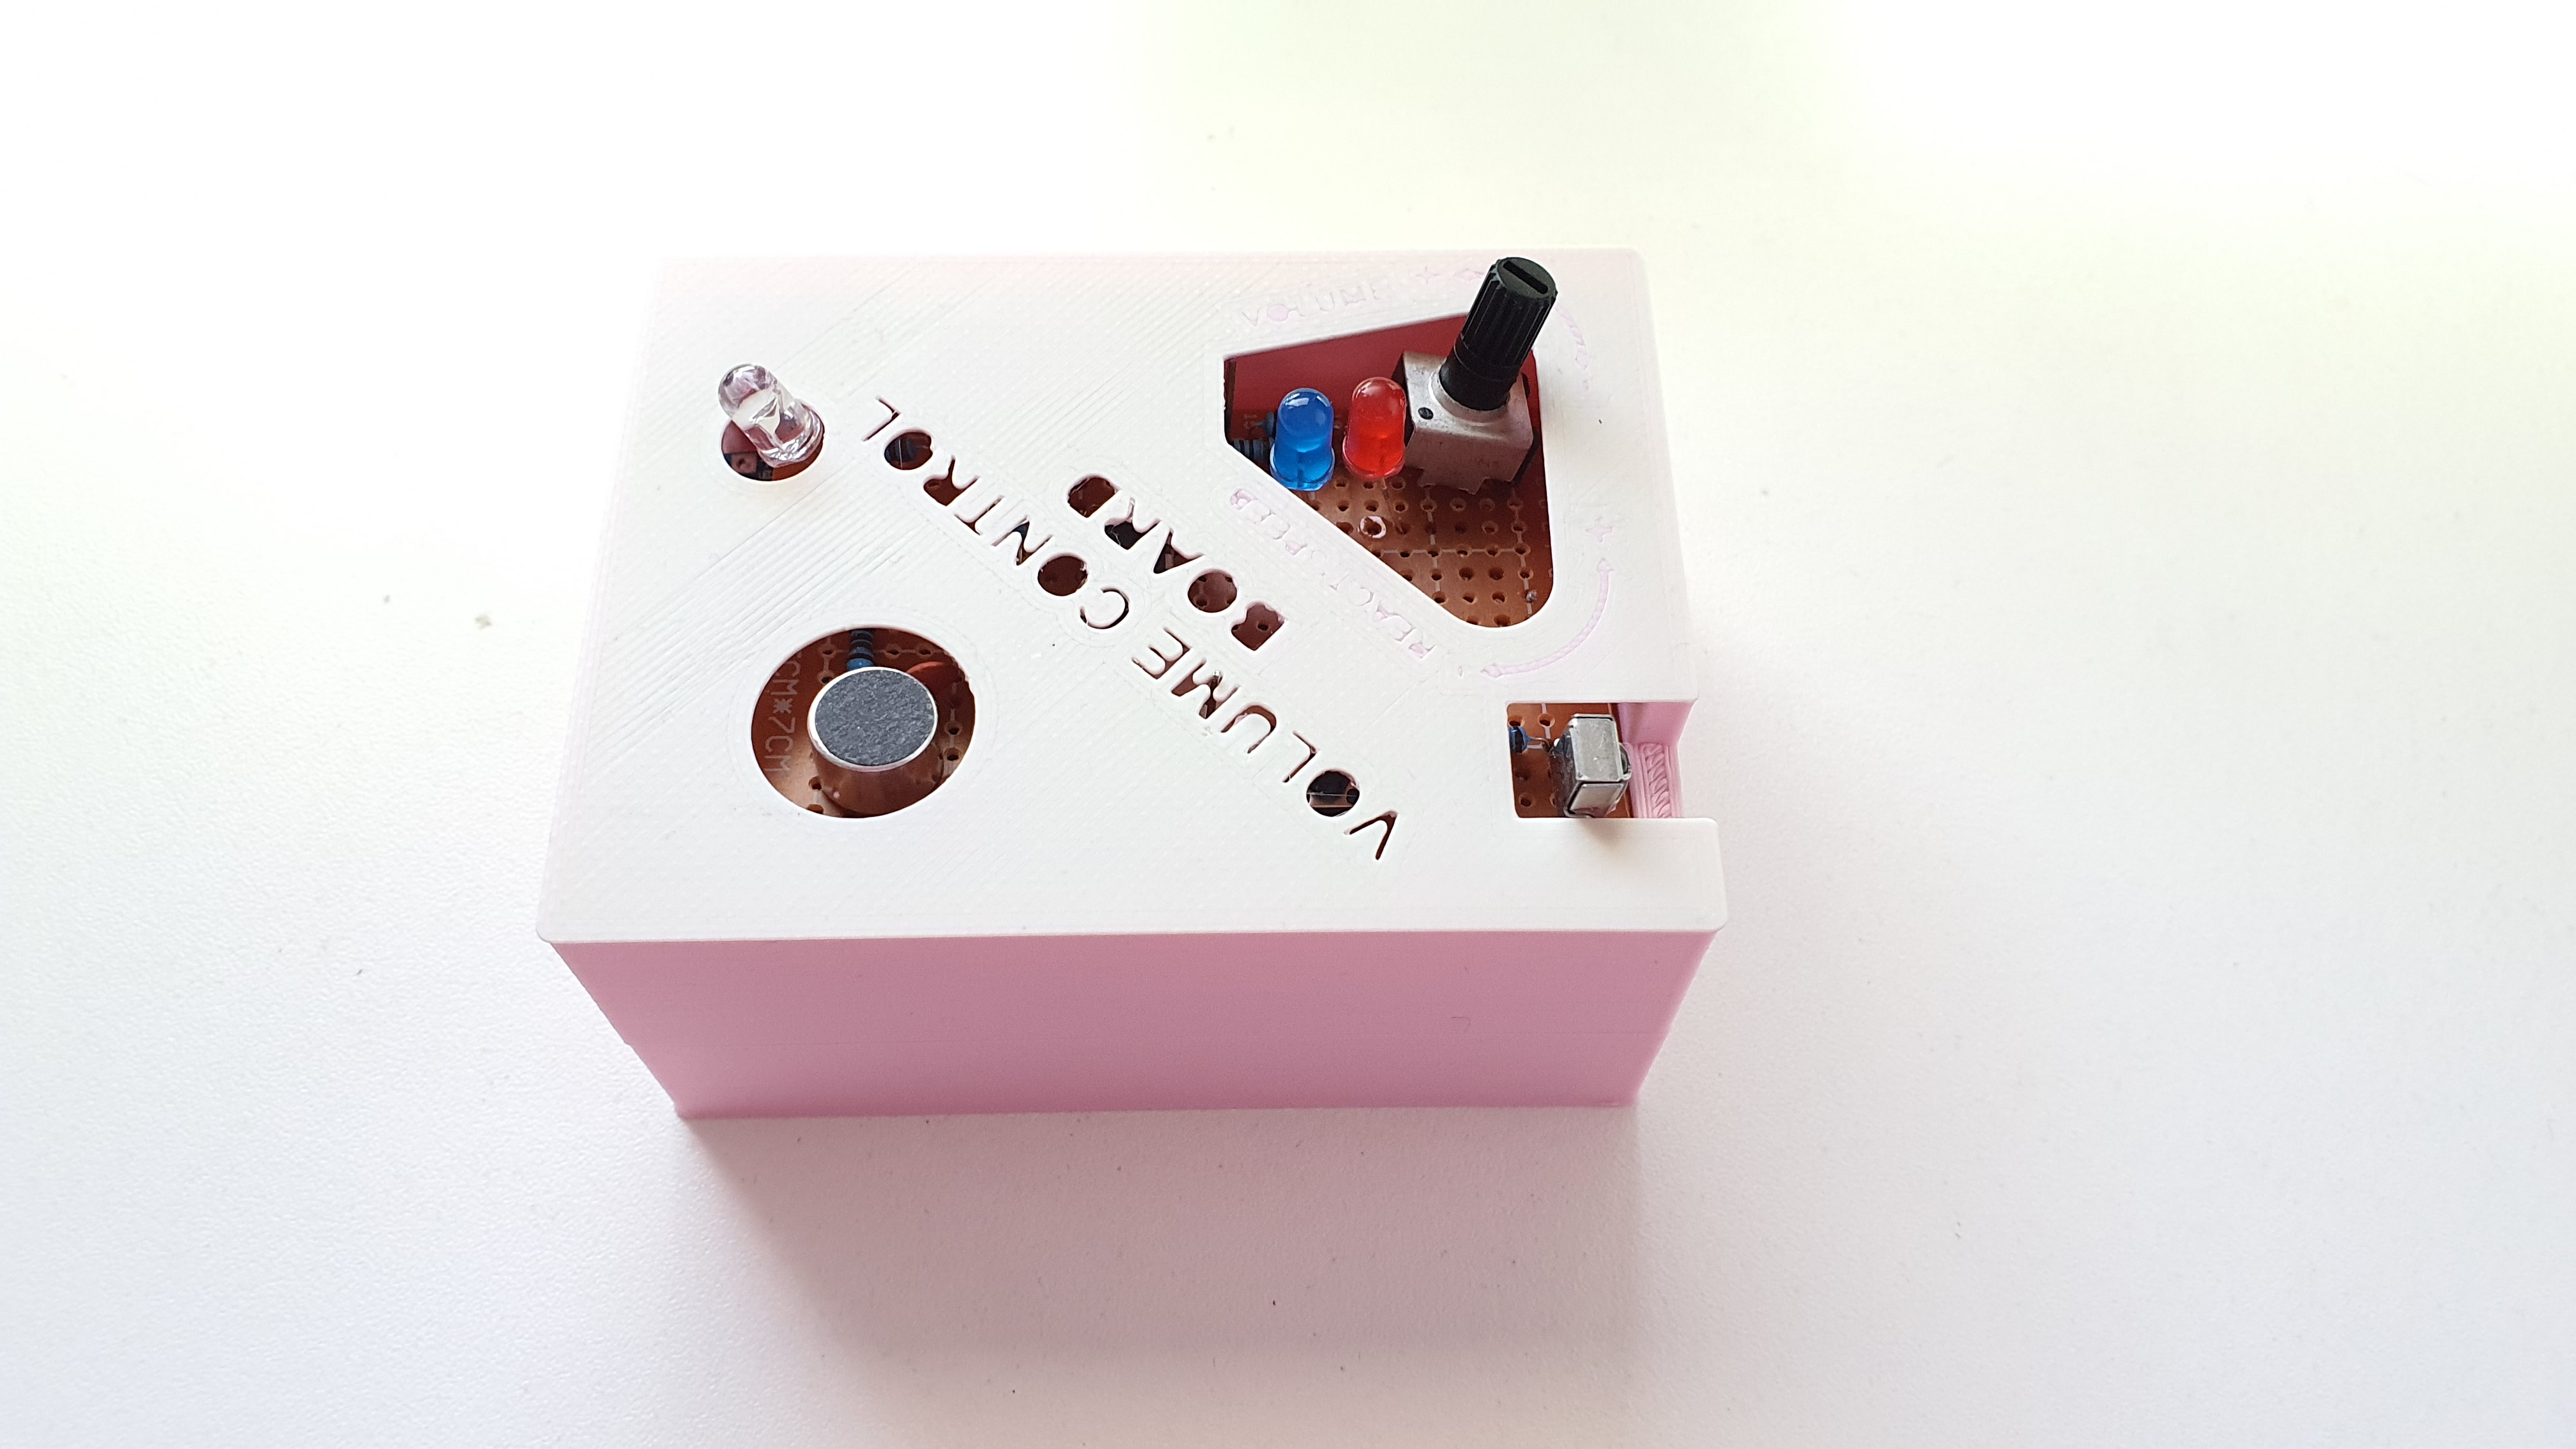
\includegraphics[width=\textwidth]{obr/obaltopuhol.jpg}}
\caption{model ovládača aj s obalom.}\label{OBRAZOK 1.5}
\end{figure}

Prototyp číslo 2 fungoval počas testovania správne a všetky funkcie sme vyladili priamo pre tento systém. Avšak pred odovzdaním projektu sa vyskytol problém so zapojením obvodov a výstupy do Arduina prichádzali v zlom tvare obr.\ref{OBRAZOK 1.8}. Problém sme odhadli na skrat medzi súčiastkami zapojenia kedy sa do výstupu mikrofónu pridával neznámy šum, ktorý znehodnotil výsledky merania mikrofónu. Chybu sme sa snažili lokalizovať a odstrániť, avšak aj napriek veľkej snahe sa nám chybu nepodarilo nájsť a opraviť.

\begin{figure}[!tbh]
\centering
\fbox{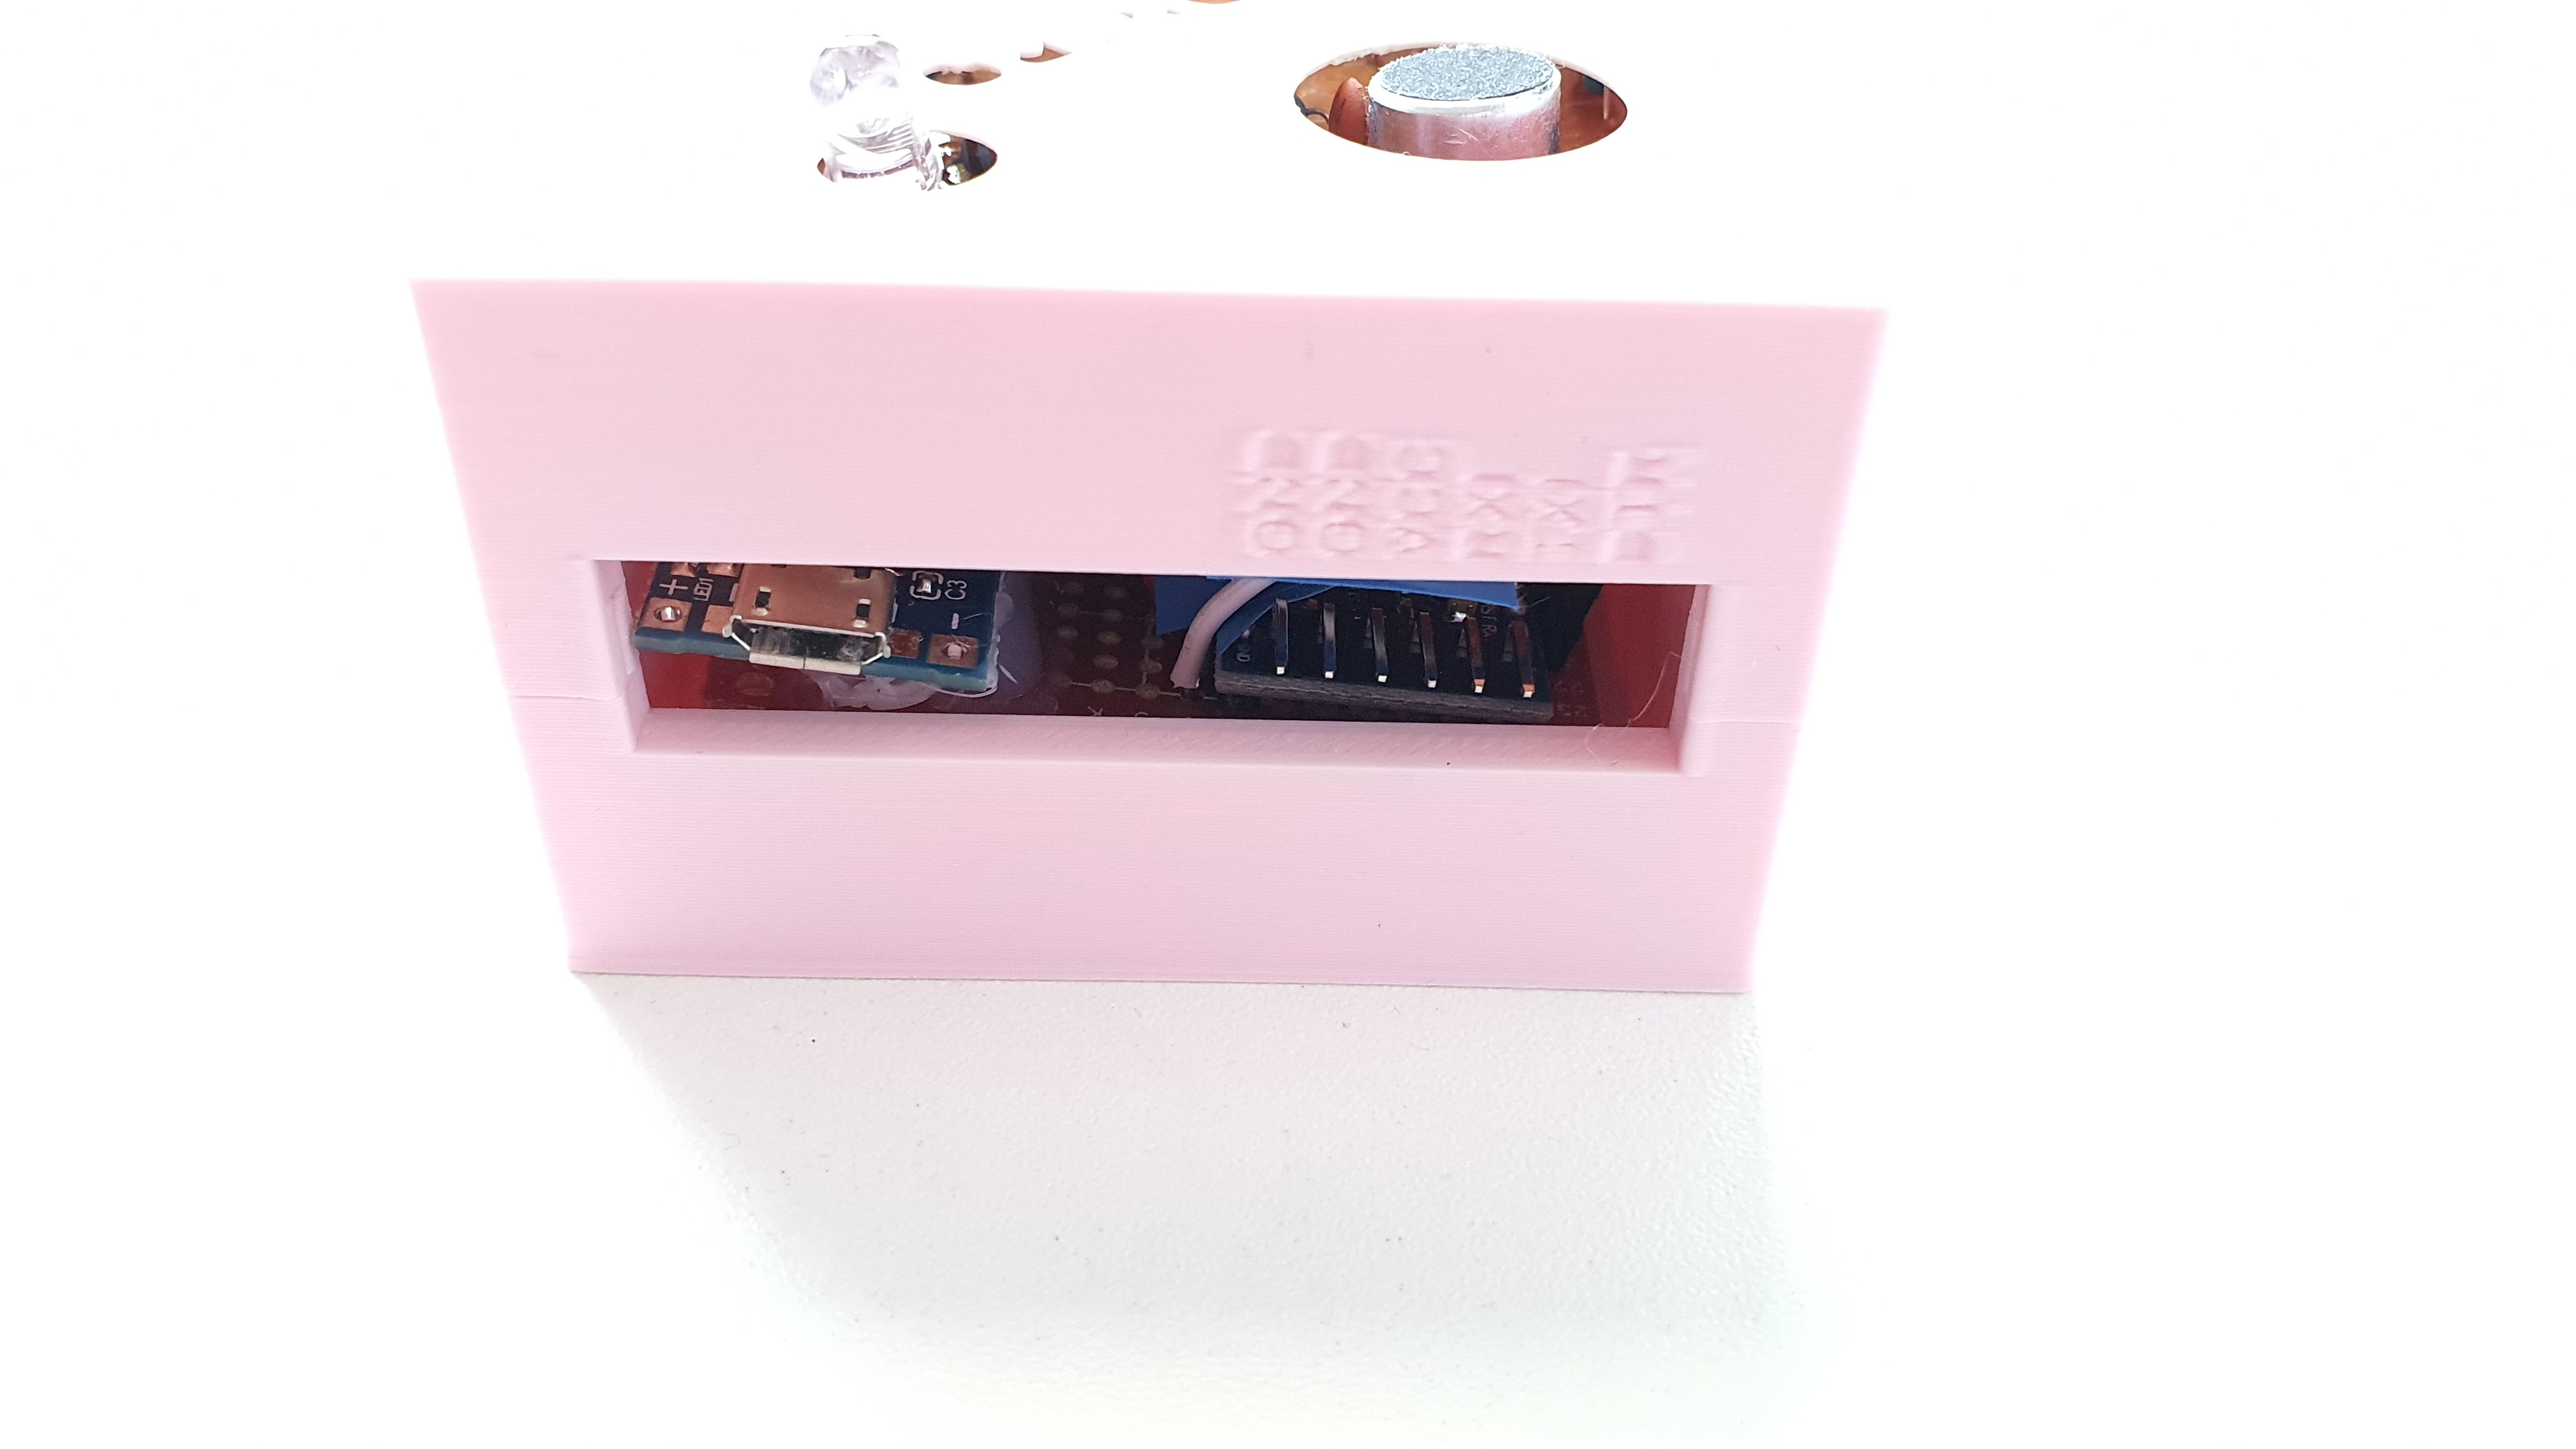
\includegraphics[width=\textwidth]{obr/obalkonektory.jpg}}
\caption{model ovládača zadná strana.}\label{OBRAZOK 1.6}
\end{figure}

\begin{figure}[!tbh]
\centering
\fbox{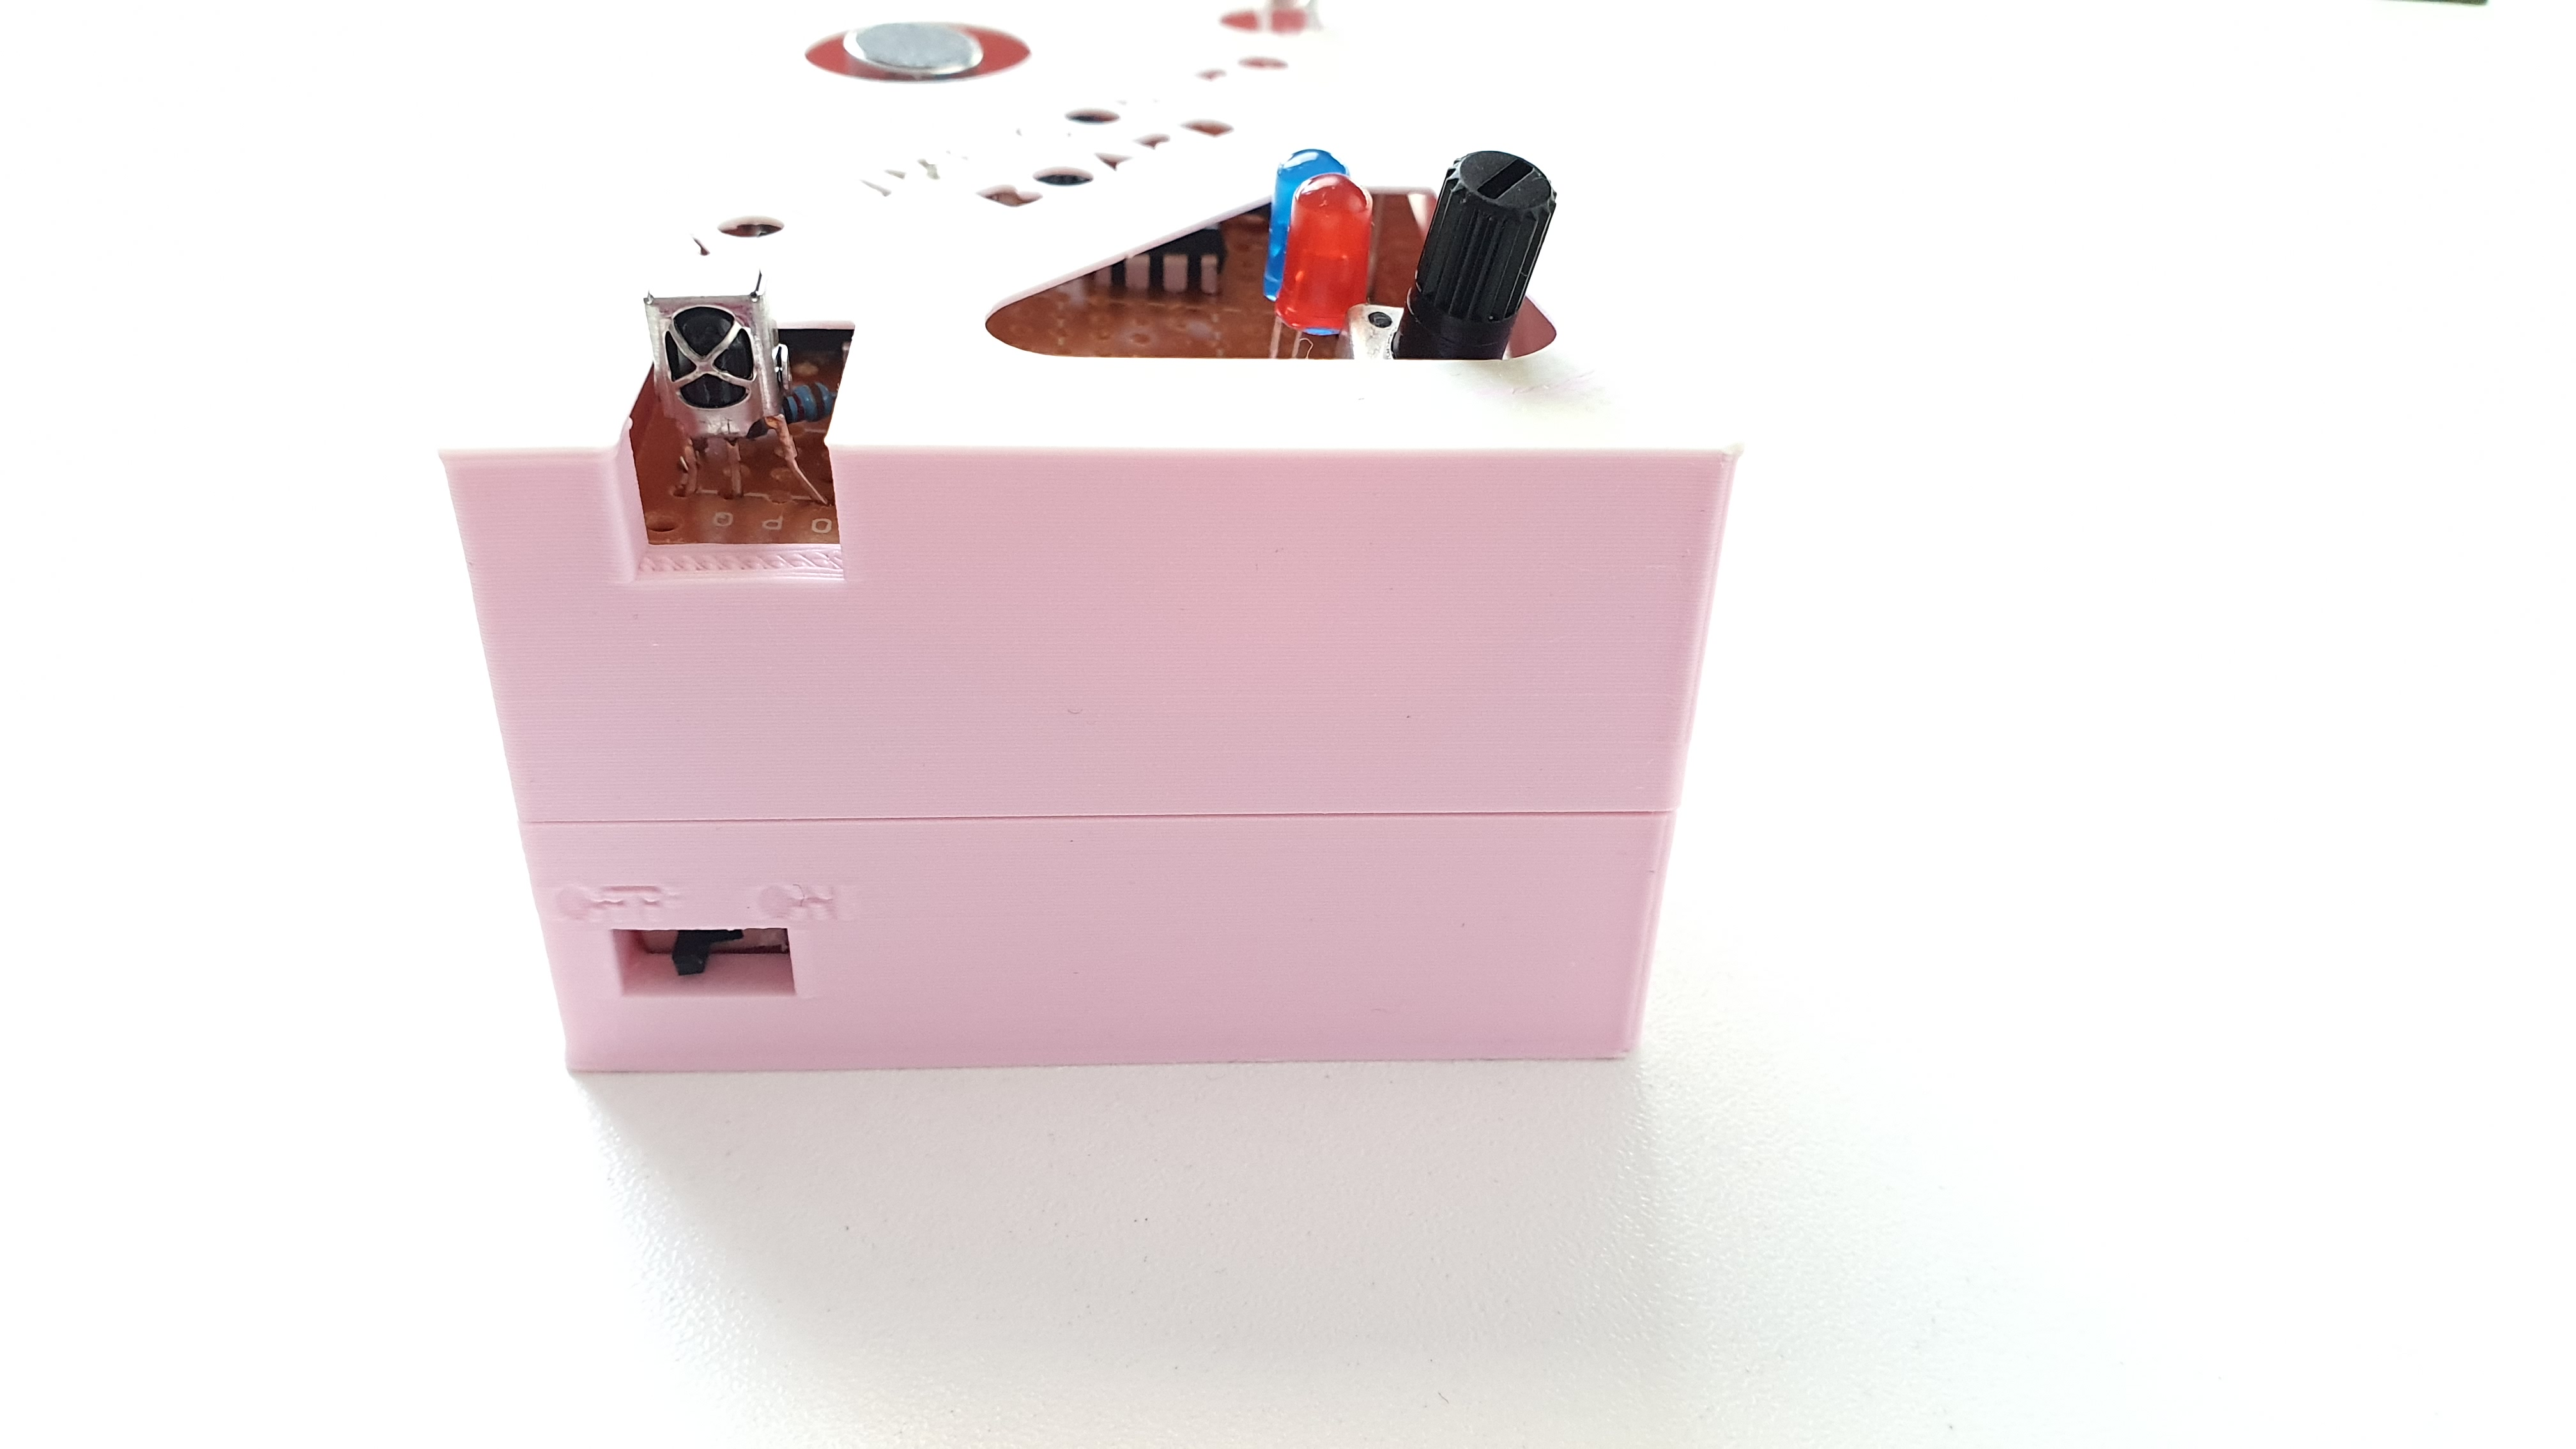
\includegraphics[width=\textwidth]{obr/obalkraj.jpg}}
\caption{model ovládača predná strana.}\label{OBRAZOK 1.7}
\end{figure}

Kvôli zabezpečeniu všetkých komponentov sme sa rozhodli vyrobiť pre náš ovládač hlasitosti aj obal ktorý bol vytlačený na 3D tlačiarni. Obal má na vrchnej strane výrezy pre všetky potrebné komponenty ako aj popisy funkcii akčných členov systému(potenciometrov). Z bočnej strany obalu je výrez pre vypínač s ktorým sa dá zariadenie vypnúť a zapnúť. Z druhej strany je výrez pre nabíjanie batérie a piny pre pripojenie Arduina ku počítaču.


\begin{figure}[!tbh]
\hfill
\subfigure[vrchná strana prototypovej dosky.]{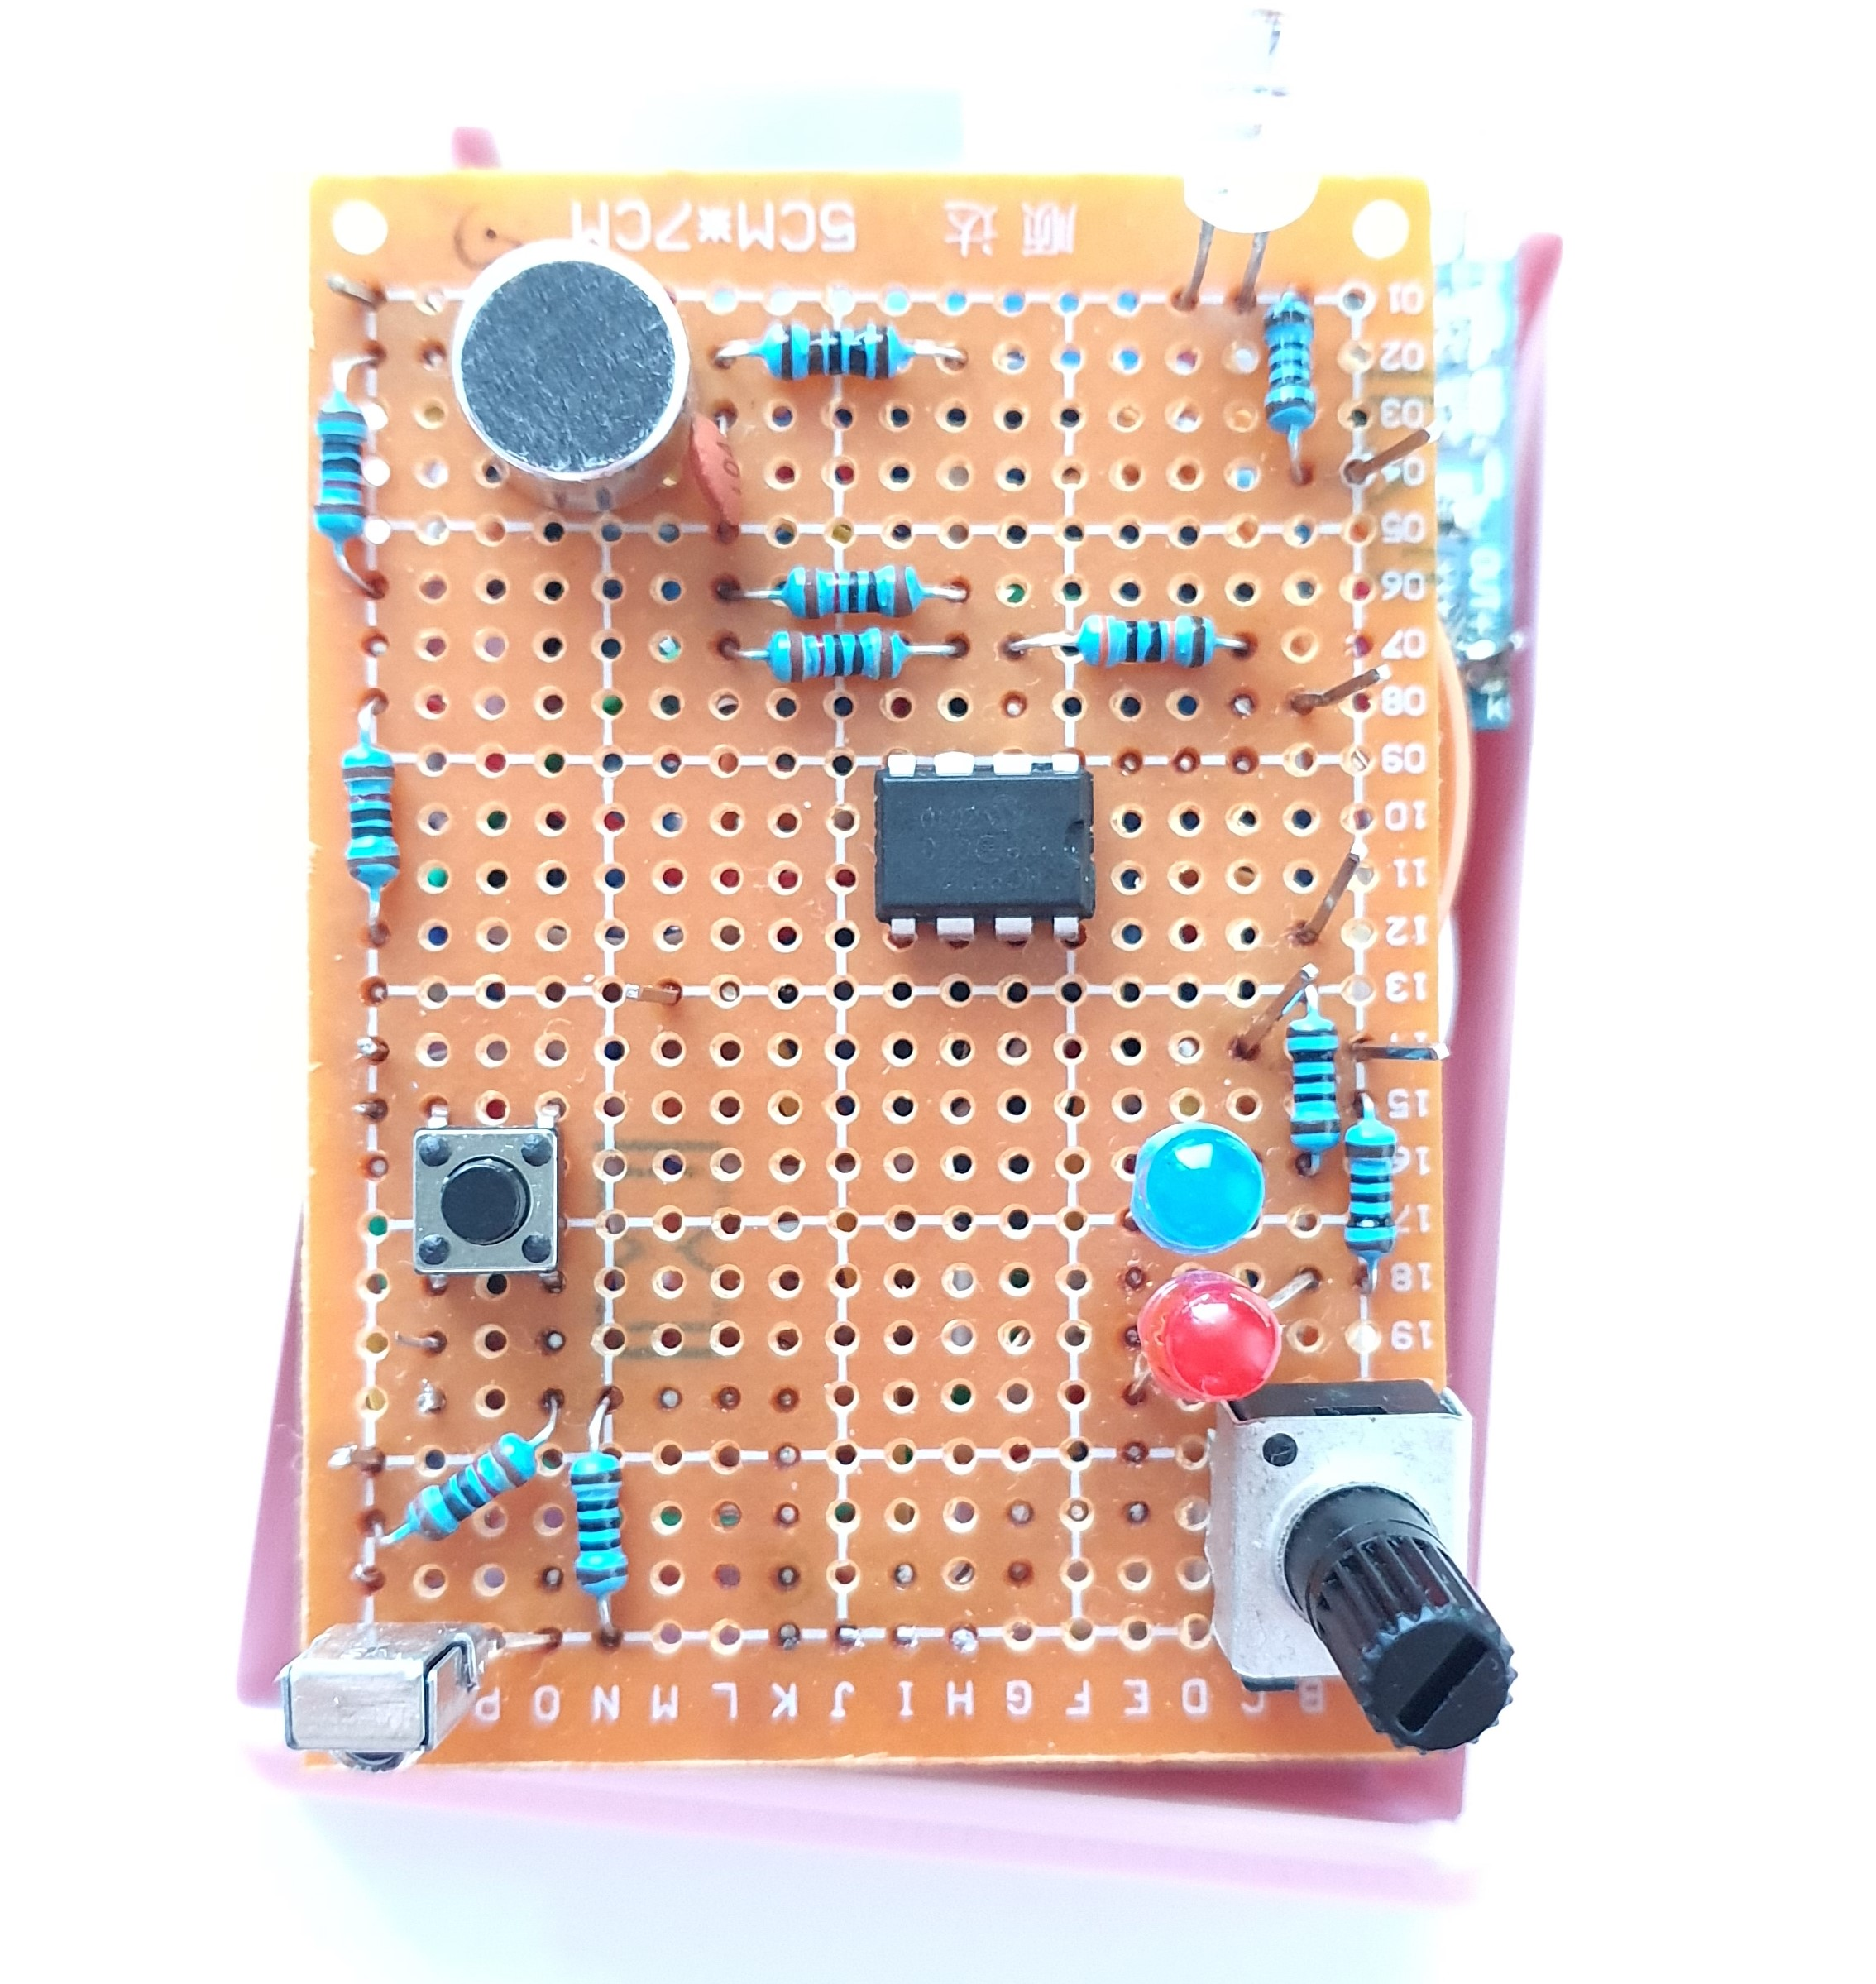
\includegraphics[width=7cm]{obr/pajkahore.jpg}}
\hfill
\subfigure[spodná strana spojov]{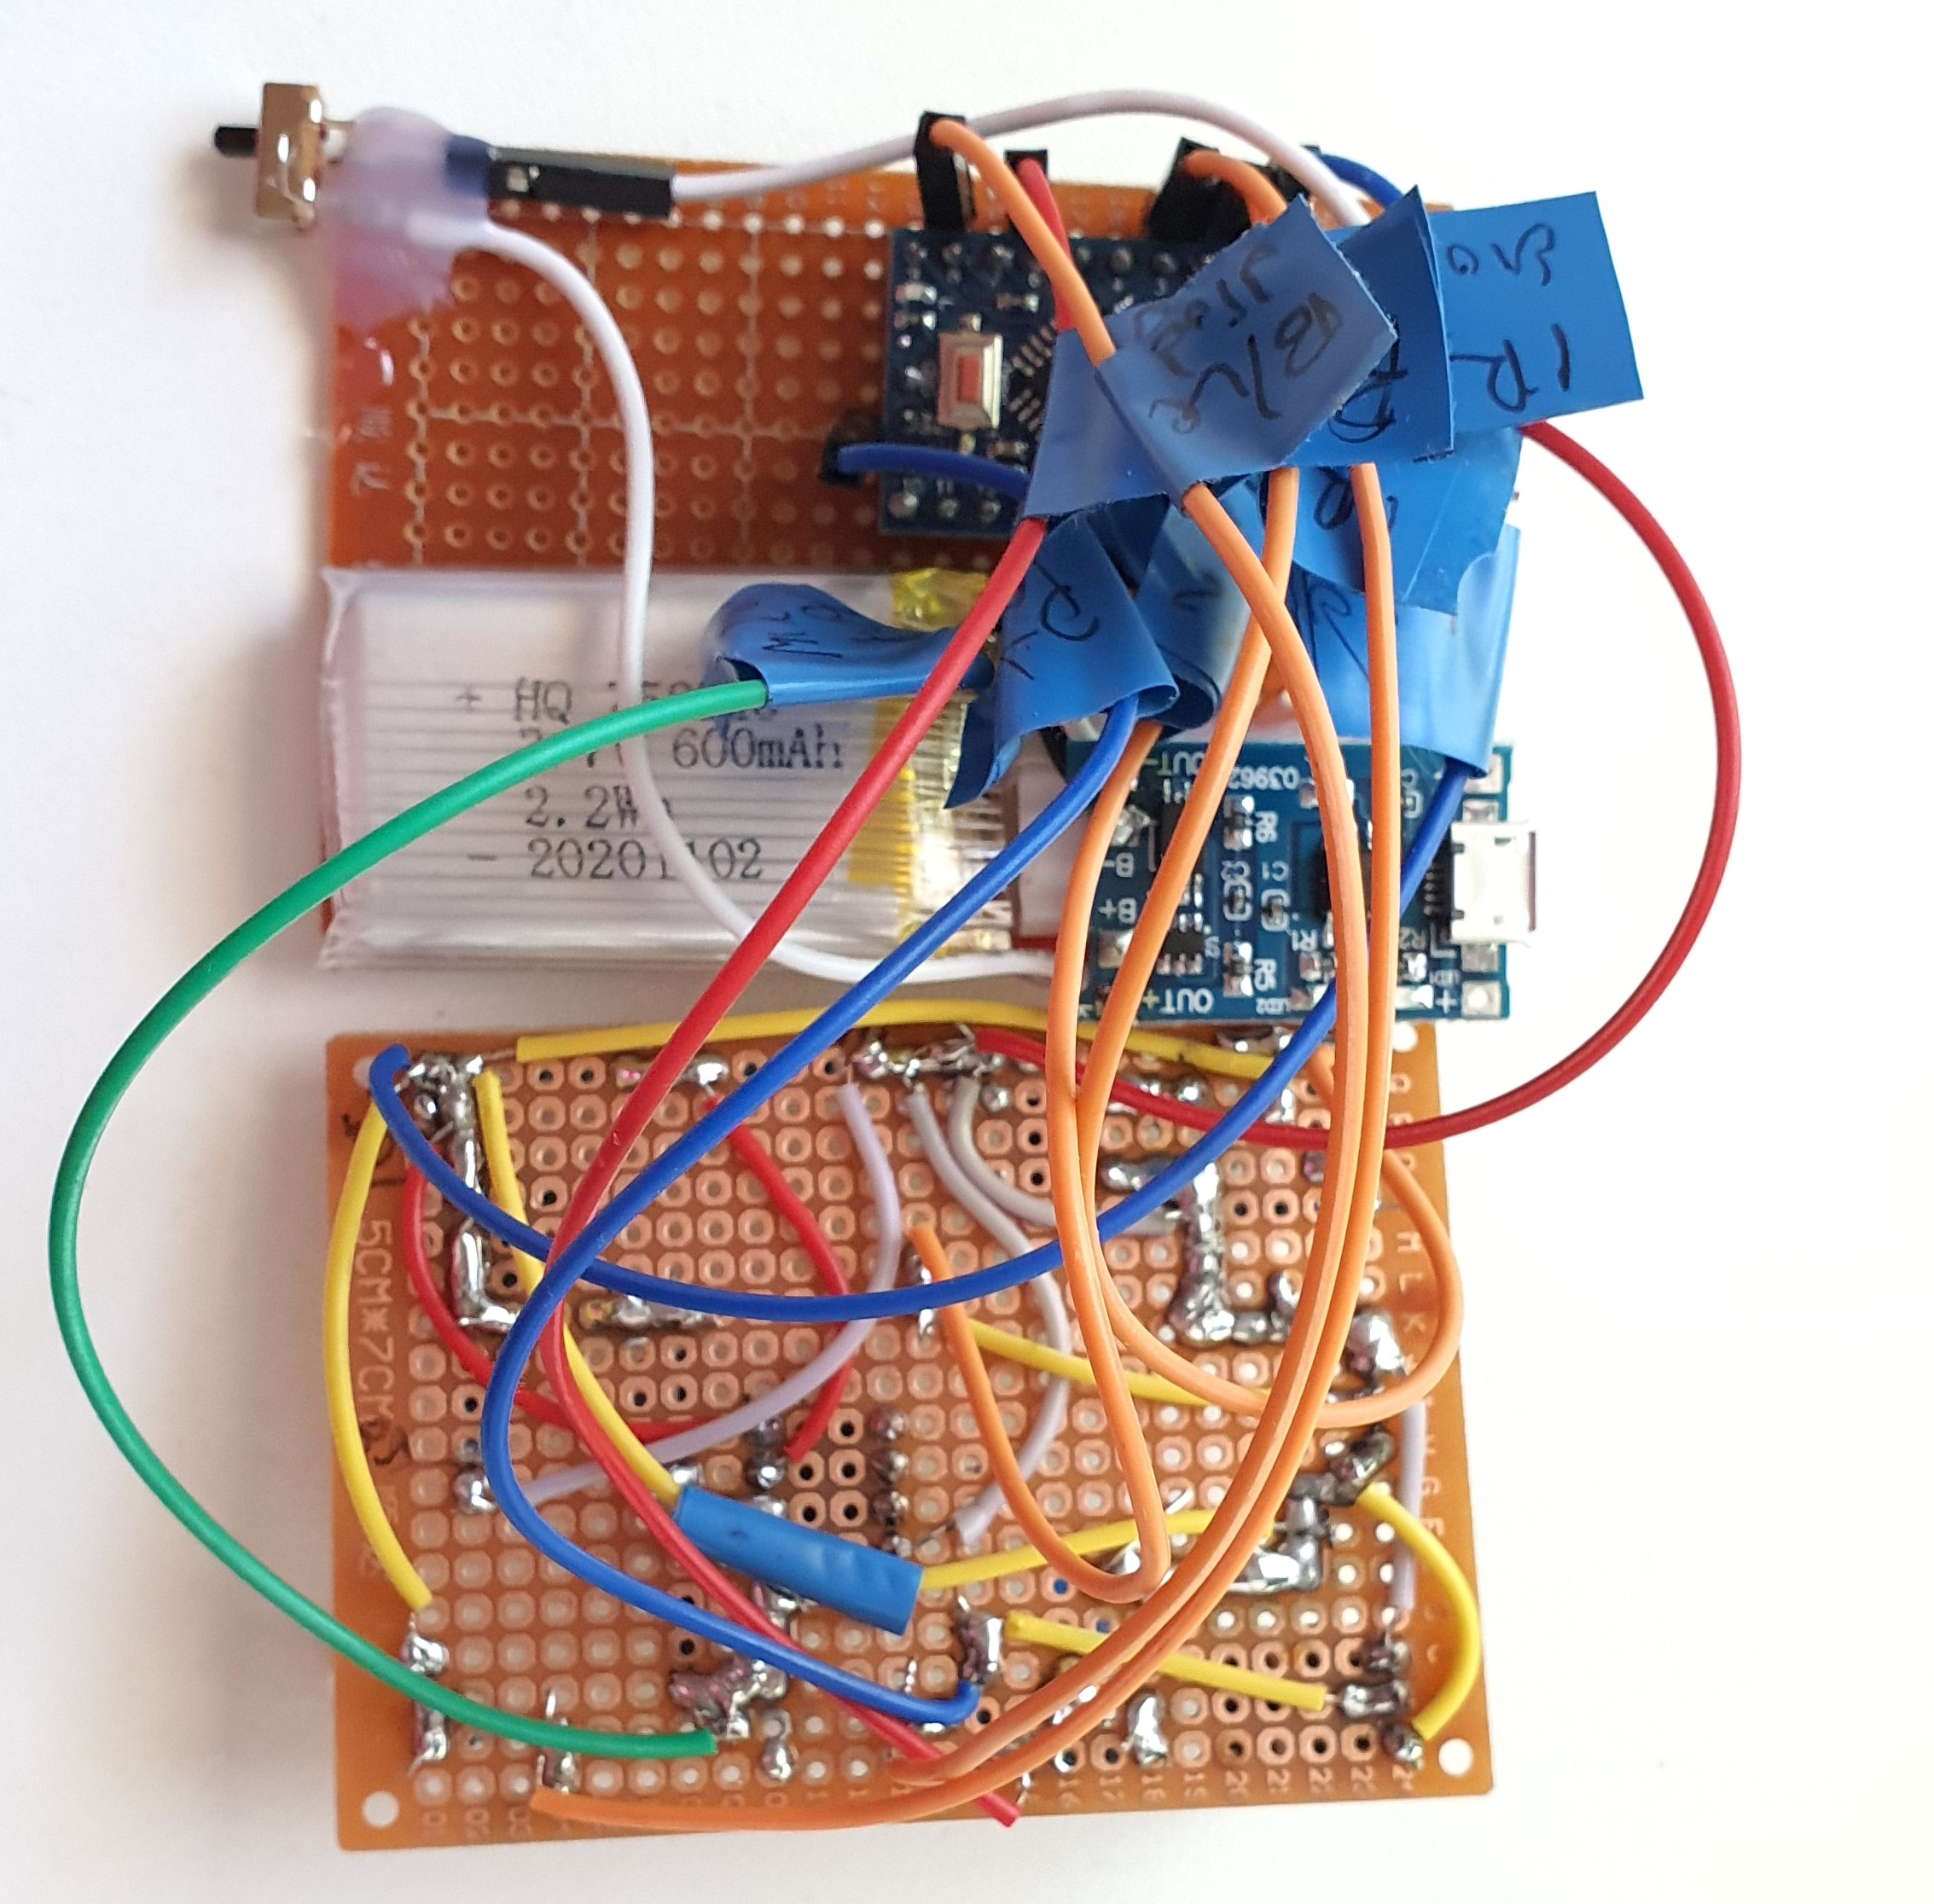
\includegraphics[width=7cm]{obr/pajkavsetko.jpg}}
\hfill
\caption{zapojenie pomocou jednostrannej prototypovej dosky}\label{OBRAZOK 1.8}
\end{figure}


